\documentclass[UTF8,a4paper,12pt,fontset=none]{ctexart}
\usepackage[margin=2.5cm]{geometry}
\usepackage{amsmath,amssymb}
\usepackage{graphicx}
\usepackage{booktabs}
\usepackage{longtable}
\usepackage{array}
\usepackage{float}
\usepackage{caption}
\usepackage{xcolor}
\usepackage{hyperref}
\usepackage{setspace}
\setCJKmainfont{Noto Serif CJK SC}
\setCJKsansfont{Noto Sans CJK SC}
\setCJKmonofont{Noto Sans Mono CJK SC}
\setstretch{1.35}
\setlength{\parskip}{0.35em}
\emergencystretch=2em
\hypersetup{
    colorlinks=true,
    linkcolor=blue,
    citecolor=blue,
    urlcolor=blue
}
\graphicspath{{../../}{../../report_assets/Report/}}

\title{ConFIG 无冲突梯度方法在物理信息神经网络训练中的优化建模与实验分析}
\author{}
\date{}

\begin{document}
\maketitle
\tableofcontents
\newpage



\section{ConFIG 与 PINN 多目标优化问题建模}

\subsection{研究背景与实际问题的数学建模}

近年来，AI4Science（人工智能驱动的科学研究）成为了计算科学领域最具革命性的发展方向之一。在传统的物理学、流体力学以及材料科学中，系统的动态演化通常由复杂的偏微分方程（Partial Differential Equations, PDEs）来描述。然而，传统的数值求解方法（如有限元法 FEM、有限差分法 FDM）高度依赖于网格划分，在面对高维问题或复杂几何边界时面临严重的“维度灾难”和巨大的计算开销。


为了解决这一问题，物理信息神经网络（Physics-Informed Neural Networks, PINNs）被提出。从数学优化的视角来看，PINNs 的本质是将传统的“微分方程求解问题”等价转化为一个“连续空间中的非凸优化问题”。


具体而言，考虑一个定义在时空域 $\Omega \subset \mathbb{R}^d$ 上的非线性 PDE 一般形式：

\[
\mathcal{F}[u(\mathbf{x}, t)] = 0, \quad (\mathbf{x}, t) \in \Omega
\]
包含边界条件（BC）和初始条件（IC）：

\[
\mathcal{B}[u(\mathbf{x}, t)] = 0, \quad (\mathbf{x}, t) \in \partial\Omega
\]
\[
u(\mathbf{x}, 0) = u_0(\mathbf{x}), \quad \mathbf{x} \in \Omega
\]

在 PINNs 的框架下，本文使用带有参数 $\theta$ 的神经网络 $u_\theta(\mathbf{x}, t)$ 来逼近真实解。根据极值原理和变分法思想，PDE 的求解被建模为一个极小化目标泛函（Objective Functional）的过程。该优化的整体损失函数（Loss Function）由三部分残差构成：

\[
\min_{\theta \in \mathbb{R}^n} \mathcal{L}(\theta) = \mathcal{L}_{PDE}(\theta) + \lambda_{BC} \mathcal{L}_{BC}(\theta) + \lambda_{IC} \mathcal{L}_{IC}(\theta)
\]

其中：

\begin{itemize}
\item $\mathcal{L}_{PDE}(\theta) = \frac{1}{N_f} \sum_{i=1}^{N_f} \| \mathcal{F}[u_\theta(\mathbf{x}_i, t_i)] \|^2$ 表示方程物理法则的残差；
\item $\mathcal{L}_{BC}(\theta)$ 和 $\mathcal{L}_{IC}(\theta)$ 分别表示边界和初始数据的拟合误差；
\item $\lambda_{BC}, \lambda_{IC} > 0$ 为惩罚系数（Penalty Coefficients）。
\end{itemize}

从优化课程视角看， 显然，上述建模将物理约束嵌入到了目标函数中。在数学优化理论中，这实际上是一个经典的无约束多目标优化问题（Unconstrained Multi-objective Optimization Problem）。传统方法通过人为设定的标量权重（$\lambda$）将其转化为单目标优化（即线性标量化方法 Linear Scalarization）。然而，在极其复杂的非凸（Non-convex）神经网络参数空间中，这种简单的标量化方法引发了极其严重的优化困难。


\subsection{核心问题：优化空间中的梯度冲突（Gradient Pathologies）}

虽然上述数学模型十分直观，但在实际使用梯度下降法（如 Adam、L-BFGS 等基于一阶或拟二阶信息的优化器）求解 $\min_\theta \mathcal{L}(\theta)$ 时，模型经常无法收敛，或者陷入高残差的局部极小值（Local Minima）。2025年最新的顶级会议（如 ICLR 2025）指出，导致这一现象的根本原因在于优化空间中的“梯度冲突（Gradient Pathologies）”。


在多目标优化理论中，假设我们有 $m$ 个相互竞争的子目标 $\mathcal{L}_i(\theta)$。在每一次迭代中，参数更新的梯度为各个子梯度的加权和：

\[
g_{total} = \nabla_\theta \mathcal{L}_{PDE} + \nabla_\theta \mathcal{L}_{BC} + \nabla_\theta \mathcal{L}_{IC}
\]

从梯度几何角度看，

从高维几何的视角来看，梯度的反方向指向了使得该目标函数下降最快的方向。如果物理方程的梯度 $g_1 = \nabla_\theta \mathcal{L}_{PDE}$ 与边界条件的梯度 $g_2 = \nabla_\theta \mathcal{L}_{BC}$ 之间夹角大于 $90^\circ$，即它们的内积（Dot Product）为负：

\[
\langle g_1, g_2 \rangle < 0
\]
那么这两个下降方向在空间中构成了冲突（Conflict）。


这种冲突会导致以下灾难性的优化后果：

\begin{enumerate}
\item 梯度抵消与震荡： 当 $g_1$ 和 $g_2$ 方向相反且模长相近时，$g_{total}$ 会趋近于 0。此时优化器误以为到达了驻点（Stationary Point），但实际上只是陷入了极度平缓的“鞍点（Saddle Point）”峡谷中，导致优化停滞（Stiffness）。
\item 目标竞争破坏物理规律： 当边界条件梯度主导时（$\|g_2\| \gg \|g_1\|$），神经网络会迅速拟合边界数据，但由于夹角为钝角，这一更新方向 $\Delta \theta = -\alpha g_2$ 使得 PDE 残差在投影方向上的方向导数为正（即 $\nabla \mathcal{L}_{PDE}^T \Delta \theta > 0$），导致物理方程的误差急剧上升，模型出现了所谓的“遗忘”现象。
\item 违背帕累托下降原则： 真正的多目标优化期望找到一个“共同下降方向（Common Descent Direction）”，使得所有目标都不变差，从而逐步逼近帕累托前沿（Pareto Front）。而粗暴的线性相加显然破坏了这一凸优化中的基本准则。
\end{enumerate}

综上， 求解物理信息神经网络的瓶颈已经不再是算力或数据，而是高度非凸空间中的多目标优化策略问题。如何利用优化算法设计出一个满足所有子梯度投影皆为正方向的严格“无冲突”梯度，是 ConFIG 等最新算法所致力于解决的核心痛点。



\subsection{课程结合点：基于凸优化理论的冲突消除（ConFIG核心思想）}

面对高度非凸且存在严重梯度的冲突的 PINN 训练空间，ICLR 2025 录用的 ConFIG 算法摒弃了传统的“动态标量权重调参”思路，转而从几何与凸优化（Convex Optimization）的视角出发，在向量空间中对梯度进行严格的数学投影与重构。这一思想与我们在课程中学习的凸锥（Convex Cone）与对偶理论高度契合。


\begin{enumerate}
\item 寻找帕累托下降方向（Pareto Descent Direction）：
\end{enumerate}
在多目标优化中，假设共有 $m$ 个损失函数（例如 $m=3$，对应 PDE、BC、IC）。在第 $t$ 步迭代中，为了保证所有目标同时不劣化，需要寻找一个参数更新方向 $d \in \mathbb{R}^n$。根据方向导数（Directional Derivative）的定义，只要 $d$ 与所有子梯度 $g_i = \nabla \mathcal{L}_i(\theta)$ 的夹角都是锐角，该方向就是一个严格的公共下降方向：

\[
\langle d, g_i \rangle > 0, \quad \forall i \in \{1, 2, \dots, m\}
\]
在几何上，所有满足 $\langle d, g_i \rangle > 0$ 的向量 $d$ 的集合，构成了一个正对偶锥（Positive Dual Cone）。只要本文的更新方向严格位于这个凸锥内部，就能保证模型朝着多目标优化的帕累托最优（Pareto Optimality）方向演化，不会出现“拆东墙补西墙”的灾难性遗忘。


\begin{enumerate}
\item 核心数学解法：伪逆矩阵与空间投影：
\end{enumerate}
为了在这个对偶凸锥中找到一个“最公平”的下降方向，ConFIG 的目标是寻找一个方向 $g_u$，使得它与所有归一化子梯度 $u_i = g_i / \|g_i\|_2$ 的内积（即投影的余弦相似度）完全相等且大于零。

令 $G =[u_1, u_2, \dots, u_m] \in \mathbb{R}^{n \times m}$ 为归一化梯度构成的矩阵。本文希望寻找的 $g_u$ 满足如下线性方程组：

\[
G^\top g_u = c \mathbf{1}_m \quad (c > 0)
\]
其中 $\mathbf{1}_m$ 是全 1 向量。由于神经网络的参数维度 $n$ 远大于损失目标数量 $m$（即 $n \gg m$），这是一个高度欠定的系统。根据课程中所学的线性代数与最优化理论，可以利用Moore-Penrose 伪逆（Pseudoinverse）求得该系统的最小范数解：

\[
g_u = (G^\top)^+ \mathbf{1}_m = G(G^\top G)^{-1} \mathbf{1}_m
\]
接着，对 $g_u$ 进行归一化： $\hat{g}_u = g_u / \|g_u\|_2$。此时，$\hat{g}_u$ 就是我们在凸集空间中找到的“理想无冲突方向”。


\begin{enumerate}
\item 最终梯度的合成：
\end{enumerate}
最后，算法将原始的物理和边界总梯度 $g_{sum} = \sum_{i=1}^m g_i$ 投影到这个理想方向上，得到最终更新所用的无冲突梯度：

\[
g_{ConFIG} = (g_{sum}^\top \hat{g}_u) \hat{g}_u
\]
通过上述严密的线性代数运算，ConFIG 将原本盲目的梯度下降，转化为了一次在参数空间中求解伪逆并进行正交投影的凸优化过程。这从数学底层保证了优化轨迹的平滑性，彻底消除了梯度冲突造成的鞍点震荡。


\subsection{ConFIG 思想的潜在应用与前景}

在深入阅读该文献并结合课程内容后，本文认为：深度学习模型（特别是 AI4Science 模型）的训练瓶颈，往往不再是网络结构的设计，而是底层非凸空间中的多目标优化问题。 将运筹学和凸优化中的数学工具（如投影映射、KKT条件、伪逆）引入到机器学习的优化器中，是一个极具潜力且优雅的研究范式。


除了求解偏微分方程（PDE），这种基于空间投影的无冲突优化思想（如 ConFIG），在以下前沿领域具有极大的潜在应用价值和广阔前景：


\begin{enumerate}
\item 计算化学与药物分子设计（AI4Chemistry）：
\end{enumerate}
    在 AI4Science 中的新药发现或分子图生成（Molecular Graph Generation）的任务中，通常是一个极度困难的多目标组合优化问题。优化目标往往相互冲突：例如，既要最小化分子的结合能（物理法则），又要最大化药物的无毒性（生物法则），同时还要保证分子容易被化学合成（化学规则，SA Score）。利用伪逆梯度投影技术，可以在训练生成模型（如扩散模型 Diffusion 或 GNN）时，消除这些跨学科规则之间的梯度打架，使得生成的候选药物严格处于帕累托前沿。


\begin{enumerate}
\item 具身智能（Embodied AI）与多模态多任务学习：
\end{enumerate}
    在自动驾驶或机器人控制系统中，模型通常需要同时输出目标检测（视觉感知）、深度估计（空间感知）以及转向控制（行为决策）。这些不同维度的任务损失处于不同的量级，导致多任务学习（Multi-task Learning, MTL）常出现“负迁移（Negative Transfer）”。将这种严谨的数学投影算法应用于多任务特征提取层的反向传播中，可以保证视觉感知不会破坏运动规划的性能，具有极大的工业落地价值。


\begin{enumerate}
\item 大语言模型（LLMs）的对齐（Alignment）与强化学习优化：
\end{enumerate}
    在强化学习（RLHF）训练大模型时，模型往往需要权衡“回答的有用性（Helpfulness）”和“无害性（Harmlessness）”。未来，可以将 ConFIG 的无冲突思想与强化学习中的策略梯度（Policy Gradient）结合，将其转化为一个双目标的受约束凸规划问题，从而避免模型为了追求高奖励而产生幻觉（Hallucination）。


目前的局限性与改进前景：

虽然基于伪逆的投影极其优美，但计算 $(G^\top G)^{-1}$ 涉及矩阵求逆操作。如果未来面临上百个冲突目标（即 $m$ 极大时），计算复杂度会骤增。未来的改进方向可以结合组合优化中的随机采样技术（Randomized Subspace Sampling）或低秩近似（Low-rank Approximation, 如 SVD 截断），在极高维的参数空间中用近似方法寻找对偶凸锥中的正方向，这将在保证优化性能的同时进一步降低算力开销。




\section{物理建模中梯度冲突消除方法的发展现状与趋势}

在深入剖析了基于多目标优化的 ConFIG 算法后，本节将聚焦于“物理建模中的梯度冲突消除与多目标优化”这一特定主题，详细梳理其国内外的研究现状、演进脉络，并结合 2025-2026 年的顶会文献（如 ICLR、NeurIPS、CVPR 等）探讨最新的发展趋势。


\subsection{物理建模优化的国内外发展现状}

在基于深度学习的偏微分方程（PDE）求解以及多任务学习（Multi-Task Learning, MTL）领域，目标函数之间存在竞争与冲突是一个长期存在的根本性痛点。为了解决这一高度非凸空间中的优化难题，国内外的研究者们经历了从“启发式标量调节”到“严格向量空间投影”的几个重要发展阶段。


第一阶段：基于经验的静态标量标量化（Static Scalarization）

早期的物理信息神经网络（如 2019 年 Raissi 等人最初提出的 PINN）以及绝大多数多模态模型，在处理多目标优化时，均采用最朴素的线性标量化策略（Linear Scalarization）。即通过人工设定的静态超参数（Hyper-parameters）将残差简单相加： $\mathcal{L} = \mathcal{L}_{PDE} + \lambda \mathcal{L}_{BC}$。

\begin{itemize}
\item 局限性： 这种方法极度依赖于专家的“炼丹”经验。由于参数空间极度不平滑（Non-smooth），微小的 $\lambda$ 变化都会导致优化器在不同的极小值域间剧烈跳跃，完全无法保证解的物理正确性。
\end{itemize}

第二阶段：基于数值信息的动态权重调节（Dynamic Weighting Era）

随着研究的深入，学术界开始尝试在训练过程中自动调节各项的相对权重，以期达到各个目标损失的平衡。这一阶段国内外涌现了大量具有代表性的启发式优化算法：

\begin{enumerate}
\item 梯度范数平衡（GradNorm）： 核心思想是在反向传播时，动态调整各项的权重 $\lambda_i$，使得所有子损失函数在同一网络层产生的梯度范数（L2-Norm）处于同一数量级，防止某一任务过早占据主导地位。
\item 神经正切核引导（NTK-guided）： 王世晓（S. Wang）等人在 2021 年的研究中，首次从极值理论和神经正切核（Neural Tangent Kernel）的角度分析了 PINN 优化的病态收敛率问题，并提出利用 NTK 的特征值来动态惩罚收敛过快的损失项。
\end{enumerate}
\begin{itemize}
\item 局限性剖析（结合优化理论）： 无论上述标量权重调节策略设计得多复杂，其本质依然是标量乘法操作（Scalar Multiplication）。在向量几何中，乘以一个正标量只能改变梯度向量的“长度（Magnitude）”，却永远无法改变梯度的“方向（Direction）”。因此，如果 $\nabla \mathcal{L}_{PDE}$ 与 $\nabla \mathcal{L}_{BC}$ 在参数空间中原本就存在超过 90 度的钝角冲突，仅仅调整大小根本无法解决梯度的相互抵消现象。
\end{itemize}

第三阶段：基于向量空间投影的多目标优化（Vector-space Projection \& MTL Era）

为了从根本上消除冲突，国内外顶尖机构（如 MIT、斯坦福大学、清华大学等）开始引入凸优化和运筹学中的帕累托最优（Pareto Optimality）思想，直接在参数的高维切空间上对梯度向量进行几何操作。这一方向成为了近两年来计算数学与 AI 交叉领域的核心热点。

\begin{enumerate}
\item PCGrad（Projecting Conflicting Gradients）： 这一算法（NeurIPS 2020）是该阶段的奠基之作。当检测到两个梯度向量 $g_i$ 和 $g_j$ 存在冲突（即内积为负）时，PCGrad 强制将其中一个梯度投影到另一个梯度的法平面（Normal Plane）上，从而人为创造出正交不冲突的更新方向。然而，它的致命弱点在于强烈的顺序依赖性（Order Dependence）：多于三个目标时，投影的先后顺序会导致最终的收敛轨迹完全不同。
\item CAGrad（Conflict-Averse Gradient Descent）： 该算法将梯度更新建模为一个局部的极大极小化问题（Minimax Problem），在一个定义好的邻域内寻找最差情况下的最优下降方向。虽然理论严密，但其计算需要求解一个复杂的二次规划（Quadratic Programming, QP）问题，计算开销极大。
\end{enumerate}

总结： 在 ConFIG 等最新算法提出之前，现有的优化方法要么无法改变冲突的本质（动态权重），要么在数学投影过程中存在次优性与高昂的计算代价（PCGrad/CAGrad）。这为 2025-2026 年基于精确线性代数（如伪逆和对偶锥）的新型无冲突优化求解器留下了广阔的发展空间。




\subsection{2025-2026年最新顶会趋势梳理与前沿进展}

随着大模型和 AI4Science 的爆发，2025 年和 2026 年的各大顶级会议（如 ICLR、ICML、CVPR 及 NeurIPS 等）在“非凸空间的多目标优化”与“复杂物理系统的约束求解”方向上，呈现出了三个极其显著的最新发展趋势：


趋势一：利用二阶优化与预条件（Preconditioning）隐式消除冲突

长期以来，深度学习高度依赖于一阶（First-order）优化器（如 Adam）。然而，最新的优化理论研究发现，由于物理方程残差的复杂性，参数空间的海森矩阵（Hessian Matrix）存在极高的条件数（Condition Number），这加剧了梯度的病态行为。

\begin{itemize}
\item 最新进展： 在 2025 年至 2026 年的研究中，研究者们开始回归经典的牛顿法（Newton's Method）与二阶优化思想。例如，一些被 ICLR 2025 录用的研究探讨了如何通过拟二阶（Quasi-Second-Order）预条件技术（如 SOAP 优化器等）对梯度进行空间变换 [2][3]。研究证明，通过向海森矩阵的逆矩阵（或其近似，如 Fisher 信息矩阵）方向进行投影，可以在不显式计算多目标惩罚项的情况下，自动对齐不同目标的下降方向。这种从几何曲率（Curvature）角度缓解梯度冲突的方法，是当前优化课程理论向深度学习落地的绝佳案例。
\end{itemize}

趋势二：基于严格数学推导的正锥投影与动量加速（Momentum-Accelerated Pareto Optimization）

正如本报告所精读的 *ConFIG* 算法（被 ICLR 2025 Spotlight 录用）[1]，学术界越来越摒弃依赖直觉的启发式算法，转而使用凸优化（Convex Optimization）中的硬核数学工具来重构优化器。

\begin{itemize}
\item 最新进展： PCGrad 虽然开创了梯度投影的先河，但其对任务顺序的敏感性使其在超过三个目标（如流体力学中的 Navier-Stokes 方程包含动量、质量和能量守恒多个残差）时极易失效。2025-2026 年的最新文献表明，利用伪逆矩阵（Pseudoinverse）同时在所有目标的公共正对偶锥（Positive Dual Cone）内寻找唯一的帕累托最优方向，已经成为解决多目标冲突的 SOTA（State-of-the-Art）基准范式 [1][4]。同时，最新的预印本（arXiv 2026）正在尝试将动量（Momentum）结合到伪逆计算中（即本文作者提到的 M-ConFIG），以此极大地降低高维矩阵求逆带来的 $O(m^3)$ 计算复杂度。
\end{itemize}

趋势三：大语言模型（LLM）与智能体（Agent）辅助的组合优化与物理建模

除了连续参数空间（Continuous Space）的优化，结合 NLP、LLM 和具身智能等前沿方向，AI4Science 中的离散组合优化（Combinatorial Optimization）也在 2025/2026 年迎来了重大突破。

\begin{itemize}
\item 最新进展： 在设计一个物理系统（如寻找最优的合金材料配比，或放置最少的传感器来重建流场）时，其本质是一个 NP-Hard 的组合优化问题。近期的 AAAI 2026 和 CVPR 等顶会文献中涌现出了一种新范式：使用 LLM Agent 作为优化求解的“启发式搜索器” [5][6]。LLM 通过理解物理公式的语义，自主编写启发式算子（Heuristic Operators），并在庞大的离散空间中进行蒙特卡洛树搜索（MCTS）或演化算法（Evolutionary Algorithms）的迭代。随后，将选定的离散结构（如分子图拓扑）固定后，再利用类似 ConFIG 的凸松弛连续优化器对具体参数进行求解。这种“宏观组合搜索（Agent）+ 微观多目标凸优化（PINNs求解器）”的双层优化架构，代表了未来构建高度复杂的物理数字孪生系统的终极方向
\end{itemize}



\section{Burgers 方程 PINN 实验复现与结果分析}

本章基于 ConFIG 官方开源代码库完成一次可复现的 PINN 训练实验。实验目标不是简单复述论文结果，而是把课程中的多目标优化、投影、正对偶锥和非凸优化病态等概念落到真实代码运行中：观察普通标量损失求和、PCGrad 梯度投影、ConFIG 无冲突梯度和 M-ConFIG 动量版本在同一 Burgers 方程任务上的收敛行为，并据此分析 PINN 训练中的梯度冲突现象。


\subsection{实验目标与应用系统说明}

物理信息神经网络（PINNs）的训练目标通常由多个损失项共同构成，例如 PDE 内部残差、边界条件和初始条件。若直接使用

\[
\mathcal{L}_{total}=\mathcal{L}_{PDE}+\mathcal{L}_{BC}+\mathcal{L}_{IC},
\]
则优化器实际使用的是各子损失梯度的线性叠加。这个处理方式在工程上最简单，但从优化几何看，它默认所有子目标的下降方向可以兼容；一旦不同子梯度之间出现负内积，整体更新方向就可能降低一个目标的同时破坏另一个目标。


ConFIG 的应用价值正体现在这里：它不再只调整标量权重，而是在参数空间中直接构造一个与各子梯度都保持正投影的更新方向。实验系统因此可以看作一个“多目标 PINN 优化器对比平台”：同一个网络、同一组采样点规模和同一学习率调度下，分别比较 Standard Adam、PCGrad、ConFIG 和 M-ConFIG 的训练轨迹。


\subsection{Burgers 方程建模与实验设置}

本实验选择一维 Burgers 方程作为验证对象：

\[
\frac{\partial u}{\partial t}+u\frac{\partial u}{\partial x}-\frac{0.01}{\pi}\frac{\partial^2 u}{\partial x^2}=0,\quad x\in[-1,1],\ t\in[0,1].
\]
其初始条件为

\[
u(x,0)=-\sin(\pi x),
\]
边界条件由代码中的 Burgers 数据采样器统一生成。Burgers 方程虽然形式简洁，但非线性对流项会造成较尖锐的解结构，因此常被用作检验 PINN 训练稳定性的基础问题。


本次实验使用仓库 \texttt{experiments/PINN} 中的官方实现，主要设置如下：


\begingroup
\small
\begin{longtable}{p{0.30\textwidth}p{0.58\textwidth}}
\toprule
项目 & 设置 \\
\midrule
运行环境 & Python 3.10.12, PyTorch 2.11.0+cu130, CUDA 可用 \\
训练任务 & \texttt{experiments/PINN/lib\_pinns/burgers} \\
网络结构 & \texttt{BurgersNet(channel\_basics=50, n\_layers=4)} \\
可训练参数量 & 10401 \\
激活函数 & \texttt{tanh} \\
内部 PDE 采样点 & 10000 \\
边界点 & 250 \\
初始点 & 250 \\
采样方法 & Latin Hypercube \\
学习率 & 初始 \texttt{1e-3}，cosine scheduler，最终 \texttt{1e-4} \\
训练轮数 & 30000 epochs \\
运行次数 & 三个随机种子，\texttt{num\_run=3} \\
损失拆分 & \texttt{n\_losses=2}，即 PDE 内部残差与“边界 + 初始条件”两项 \\
\bottomrule
\end{longtable}
\endgroup


本次实验采用与官方 Burgers 配置一致的 30000 epochs 长训练，并对每种方法运行三个随机种子。训练使用 \texttt{tools/Report/run\_burgers\_experiments.py} 并行调度四种优化方法，结果由 \texttt{tools/Report/analyze\_burgers\_results.py} 统一读取 TensorBoard 记录、加载模型权重并在真实仿真数据 \texttt{simulation\_data.npy} 上重新计算 MSE。这样可以避免只根据训练终端输出判断效果，也能报告均值和标准差。


\subsection{对比方法与 ConFIG 实现机制}

本实验比较四类优化策略：


\begin{enumerate}
\item Standard Adam：直接将 PDE 残差损失与边界/初始条件损失相加，再调用普通反向传播。这是 PINN 中最常见的基线做法。
\item PCGrad：当两个任务梯度存在负内积时，将冲突分量投影到另一梯度的法平面上，属于启发式梯度手术方法。
\item ConFIG：分别计算各损失项梯度，并构造一个无冲突方向，使最终更新方向对各子梯度具有正投影。
\item M-ConFIG：在 ConFIG 的共同下降方向思想上引入动量缓存，用于降低反复计算多目标梯度方向带来的额外开销。
\end{enumerate}

ConFIG 的代码核心位于 \texttt{conflictfree/grad\_operator.py}。在 \texttt{n\_losses=2} 时，代码会调用 \texttt{ConFIG\_update\_double} 的简化形式；在更多损失项时，则使用最小二乘或伪逆求解共同方向。其思想可以概括为：


\[
g_{ConFIG}=\left(\sum_{i=1}^{m}g_i^\top g_u\right)g_u,
\]

其中 $g_u$ 是由归一化子梯度矩阵计算出的共同下降方向。与动态权重法不同，ConFIG 改变的是更新向量的方向，而不只是改变损失项前面的系数。


\subsection{实验结果展示}

本次实验生成的验证损失曲线如下。


\begin{figure}[H]
\centering
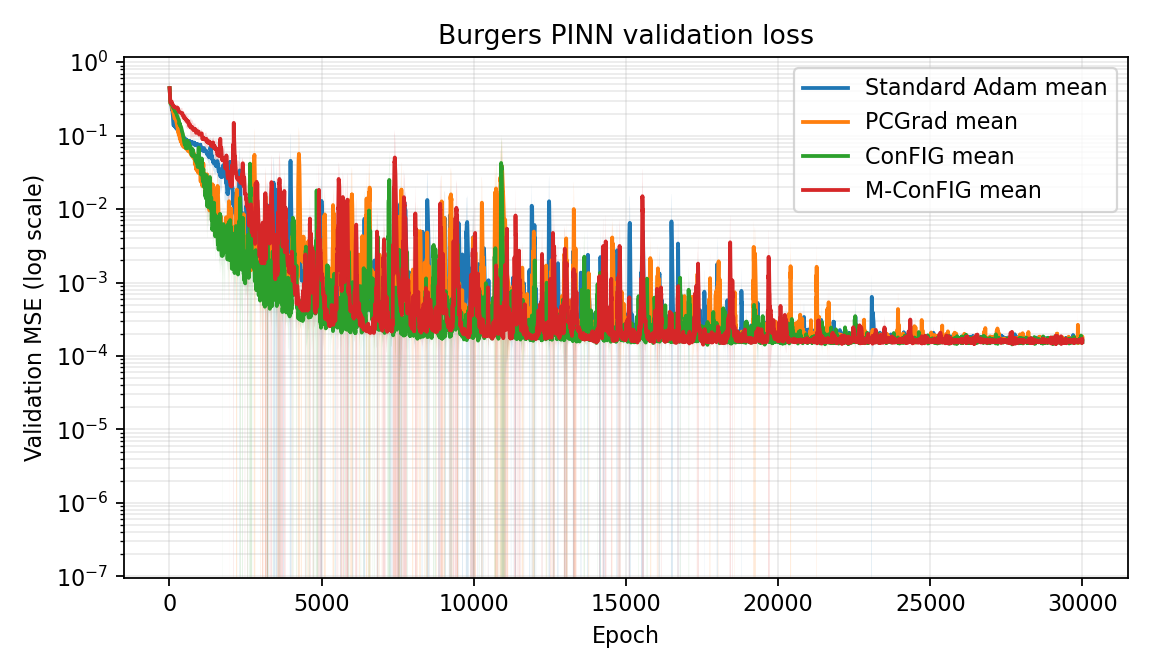
\includegraphics[width=0.92\textwidth]{../../report_assets/Report/burgers_validation_loss.png}
\caption{Burgers PINN validation loss}
\end{figure}


图 1：四种优化方法在 Burgers PINN 任务上的 validation MSE 曲线，纵轴为对数尺度。


预测解与误差热力图如下。


\begin{figure}[H]
\centering
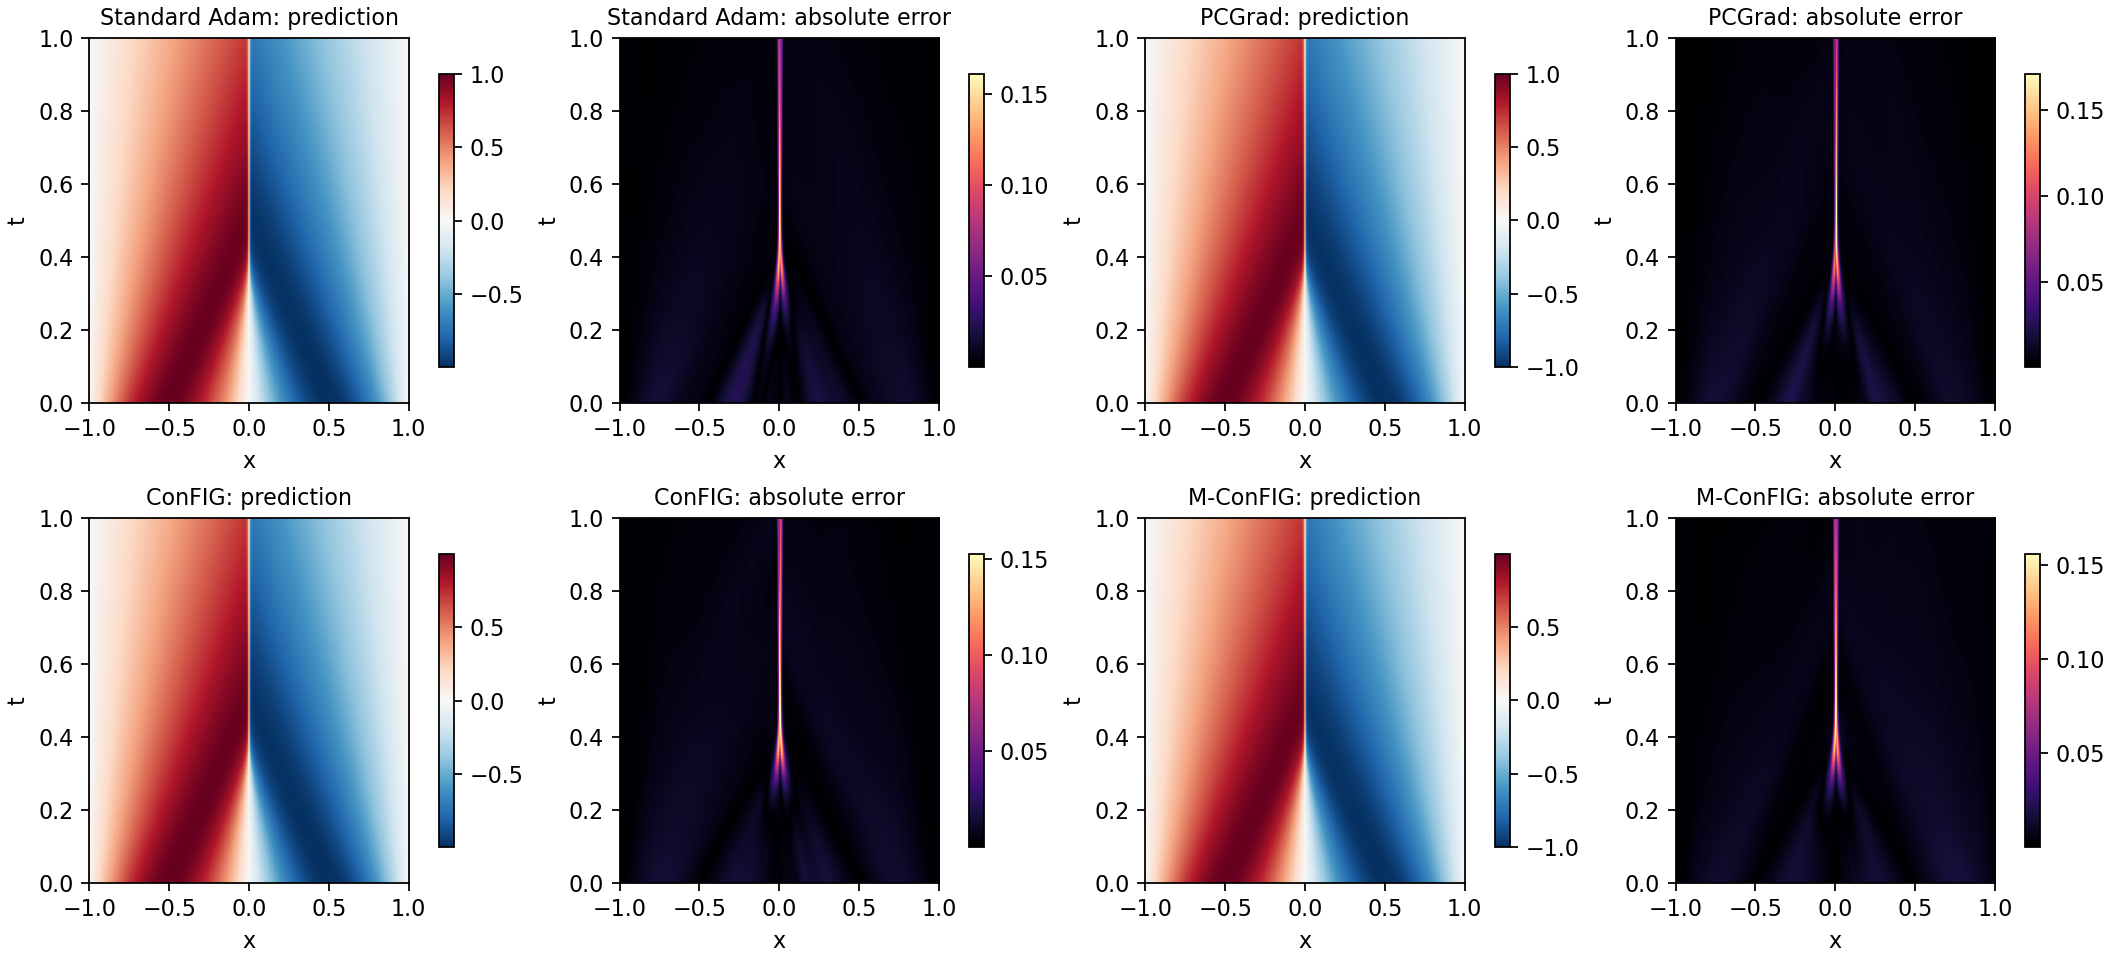
\includegraphics[width=0.92\textwidth]{../../report_assets/Report/burgers_predictions_errors.png}
\caption{Burgers predictions and errors}
\end{figure}


图 2：四种方法训练 30000 epochs 后的代表性预测解与绝对误差分布。


参考真实解如下。


\begin{figure}[H]
\centering
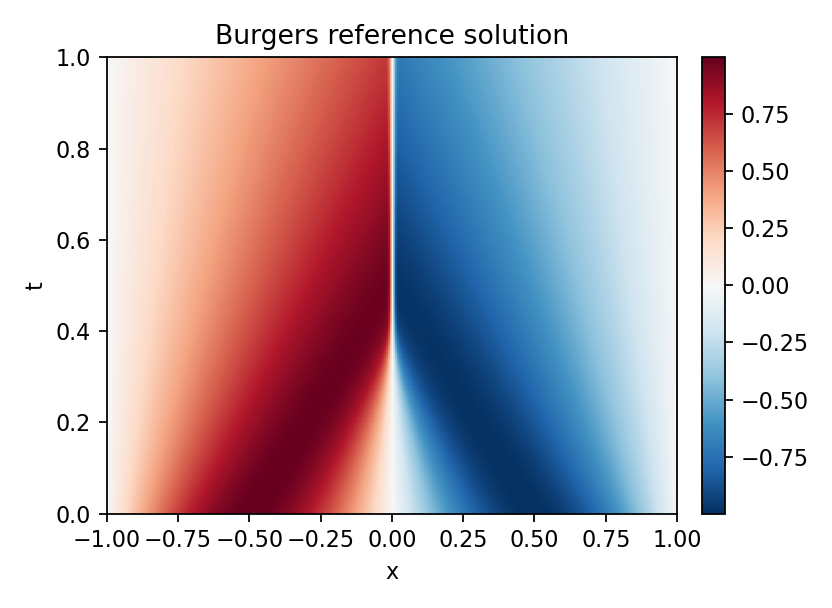
\includegraphics[width=0.92\textwidth]{../../report_assets/Report/burgers_reference_solution.png}
\caption{Burgers reference solution}
\end{figure}


图 3：Burgers 方程真实数值解。


核心数值结果如下表。MSE 来自训练结束后使用 \texttt{run\_test} 在真实仿真数据 \texttt{simulation\_data.npy} 上重新评估，表中数值为三个随机种子的均值和标准差。


\begingroup
\footnotesize
\begin{longtable}{p{0.12\textwidth}p{0.14\textwidth}p{0.14\textwidth}p{0.14\textwidth}p{0.14\textwidth}p{0.14\textwidth}}
\toprule
方法 & 最终 validation MSE & 最优 validation MSE & \texttt{run\_test} MSE & 最终 train loss & 训练速度 s/iter \\
\midrule
Standard Adam & 1.6799e-04 ± 1.1400e-05 & 1.4650e-04 ± 5.9984e-06 & 1.6799e-04 ± 1.1400e-05 & 8.9882e-05 ± 3.5693e-05 & 0.01254 ± 0.00095 \\
PCGrad & 1.7527e-04 ± 2.2738e-05 & 1.3391e-04 ± 1.5436e-06 & 1.7527e-04 ± 2.2738e-05 & 1.6994e-04 ± 1.3443e-04 & 0.01969 ± 0.00305 \\
ConFIG & 1.5516e-04 ± 5.1134e-06 & 1.3176e-04 ± 5.2519e-07 & 1.5516e-04 ± 5.1134e-06 & 1.2890e-04 ± 3.7311e-05 & 0.02033 ± 0.00381 \\
M-ConFIG & 1.5714e-04 ± 6.9572e-06 & 1.2801e-04 ± 4.2173e-06 & 1.5714e-04 ± 6.9572e-06 & 1.4448e-04 ± 2.5756e-05 & 0.01367 ± 0.00013 \\
\bottomrule
\end{longtable}
\endgroup


此外，本实验在每种方法的代表性最优 run 上，用同一组采样点重新计算 PDE 内部残差梯度与边界/初始条件梯度之间的余弦相似度，得到如下结果：


\begingroup
\small
\begin{longtable}{p{0.18\textwidth}p{0.21\textwidth}p{0.21\textwidth}p{0.21\textwidth}}
\toprule
方法 & PDE loss & BC/IC loss & 梯度余弦相似度 \\
\midrule
Standard Adam & 6.0944e-05 & 9.1503e-06 & -0.0581 \\
PCGrad & 6.3854e-05 & 5.8666e-06 & 0.0290 \\
ConFIG & 8.4620e-05 & 3.8161e-06 & -0.2620 \\
M-ConFIG & 1.4978e-04 & 3.7416e-06 & 0.6344 \\
\bottomrule
\end{longtable}
\endgroup


这个结果说明，经过 30000 epochs 的充分训练后，各方法在最终代表性模型上的梯度关系已经不再都表现为极端负相关，但仍存在明显差异：ConFIG 的代表性模型仍显示 PDE 与 BC/IC 梯度之间存在负夹角，M-ConFIG 则表现为更强的正对齐。结合训练曲线可以看到，梯度冲突不是一个固定不变的常数，而会随着优化轨迹、采样点更新和方法本身的方向修正不断变化。


\subsection{基于优化理论的实验分析}

第一，从最终验证误差看，ConFIG 在三随机种子均值上取得最低的最终 MSE，M-ConFIG 次之，Standard Adam 与 PCGrad 略高。若看训练过程中的最优 validation MSE，M-ConFIG 的均值最低，ConFIG 和 PCGrad 也明显优于 Standard Adam。这说明在充分训练下，共同下降方向或投影修正确实能改善 Burgers PINN 的优化质量，但最终排序仍会受到随机种子、采样点更新和训练末端波动影响。


第二，从梯度余弦相似度看，训练结束时不同方法的代表性模型呈现出不同的目标关系。Standard Adam 的梯度夹角接近正交，PCGrad 略为正相关，ConFIG 仍存在一定负相关，而 M-ConFIG 呈现较强正相关。这并不意味着 ConFIG 的设计失效，而是说明最终某一批采样点上的余弦相似度只能反映局部状态；真正重要的是整个训练过程中更新方向是否能够避免持续破坏任一子目标。若使用 Standard Adam，总梯度始终近似为 $g_{PDE}+g_{BC/IC}$，仍可能在冲突阶段发生抵消或互相拉扯。


第三，ConFIG 和 M-ConFIG 的结果具有重要方法论意义。PCGrad 的投影结果与任务顺序和局部启发式规则相关，而 ConFIG 的目标是构造一个对所有损失项更公平的公共方向。当损失项数量从 2 增加到 3，或者扩展到 Navier-Stokes 等包含更多物理约束的 PDE 时，ConFIG 的正对偶锥思想比简单 pairwise 投影更具有系统性。本次实验中，M-ConFIG 在最优 validation MSE 上表现最好，同时训练速度接近 Standard Adam，说明动量化方向缓存是一个值得进一步研究的效率改进方向。


第四，从训练速度看，Standard Adam 每步约 0.01254 秒，ConFIG 与 PCGrad 约为 0.02033 秒和 0.01969 秒，额外开销来自分别反向传播多个损失项以及执行梯度向量运算。M-ConFIG 每步约 0.01367 秒，明显接近 Standard Adam，同时保持了较好的最优验证误差。这也自然引出第 4 章的改进方向：如何用动量缓存、低秩近似或冲突感知的目标拆分来降低 ConFIG 的计算代价。


综上，本章实验展示了不同梯度处理方法在 Burgers 方程上的完整训练行为。对本课程而言，最重要的结论是：PINN 的训练不是一个普通的“深度学习调参问题”，而是一个典型的非凸多目标优化问题；理解梯度之间的几何关系，是设计稳定 AI4Science 训练系统的关键。




\section{方法反思、改进设想与课程总结}

通过前文的文献阅读、发展现状梳理和 Burgers 方程实验可以看到，ConFIG 最值得关注的地方，并不只是“又提出了一个新的 PINN 优化器”，而是它把深度学习训练中的经验性调参问题重新表述为一个清晰的优化几何问题：当多个损失项的梯度发生冲突时，优化器应该寻找共同下降方向，而不是只在损失权重上反复试错。


\subsection{主要结论：从调权重到构造方向}

传统 PINN 训练通常把 PDE 残差、边界条件和初始条件加权求和。这种方式隐含了一个很强的假设：各损失项梯度方向大体一致，至少不会严重冲突。但第 3 章的实验显示，不同方法在 Burgers 方程训练末端会形成明显不同的梯度几何关系，ConFIG 的代表性模型仍存在负梯度夹角，而 M-ConFIG 则表现出更强的正对齐。此时继续讨论某个 $\lambda$ 应该设为多少，实际上只能改变梯度长度，无法从根本上解释方向冲突与方向修正机制。


ConFIG 的价值在于，它将优化器设计从“标量权重选择”推进到“向量方向构造”。从课程知识角度看，这与凸锥、投影、伪逆和帕累托下降方向都有直接联系。只要最终更新方向与每个子梯度都保持正内积，就可以避免某个子目标在一步更新中被主动破坏。这种思想比单纯的经验调参更接近优化理论本身。


\subsection{当前方法的局限性}

ConFIG 目前仍有四个值得改进的问题。


第一，计算开销较高。ConFIG 需要分别对多个损失项反向传播，并保存对应梯度向量。当损失项数量很多，或者网络规模很大时，显存和时间成本都会上升。第 3 章中 ConFIG 的单步时间也高于 Standard Adam。


第二，数值稳定性依赖梯度矩阵质量。当多个损失项梯度高度共线或接近零向量时，伪逆或最小二乘求解可能变得不稳定。虽然代码中已有归一化、简化两目标求解等处理，但复杂 PDE 场景下仍可能需要更稳健的正则化。


第三，目标拆分方式会影响优化行为。比如 Burgers 任务中可以使用 \texttt{n\_losses=2}，把边界和初始条件合并；也可以使用 \texttt{n\_losses=3}，将 PDE、边界、初始条件分开。不同拆分方式会改变梯度矩阵，也会改变 ConFIG 找到的共同方向。


第四，不同统计口径可能呈现不同结论。第 3 章中 ConFIG 的最终 MSE 均值最低，而 M-ConFIG 的最优 validation MSE 均值最低；PCGrad 的最优误差也优于 Standard Adam，但最终误差波动更大。因此，改进算法时必须同时重视最终误差、最优误差、方差和单步耗时，而不能只凭一次曲线或单一指标下结论。


\subsection{改进想法一：冲突感知的动态目标拆分}

第一个改进想法是设计一种“冲突感知的动态目标拆分”机制。其核心思想是：不固定使用 \texttt{n\_losses=2} 或 \texttt{n\_losses=3}，而是在训练过程中根据梯度夹角动态决定是否合并或拆分损失项。


具体来说，可以每隔若干 epoch 计算 $\nabla \mathcal{L}_{PDE}$、$\nabla \mathcal{L}_{BC}$ 和 $\nabla \mathcal{L}_{IC}$ 两两之间的余弦相似度。如果 BC 与 IC 的梯度方向高度一致，就将二者合并，减少计算量；如果二者也出现明显负相关，则拆分为三个目标，让 ConFIG 分别处理。这样可以在“优化精细度”和“计算效率”之间取得折中。


这个方案对应课程中的组合优化思想：损失项如何分组，本质上是一个小规模离散决策问题；每一种分组又对应一个连续优化问题。未来可以把目标分组视为上层组合搜索，把 ConFIG 视为下层连续优化器，形成双层优化框架。


\subsection{改进想法二：低秩近似与动量缓存的高效 ConFIG}

第二个改进方向是降低 ConFIG 的梯度计算成本。官方代码已经提供 M-ConFIG 这类动量思路，即不在每一步都完整计算所有损失项梯度，而是缓存历史梯度信息，并按一定频率更新部分目标。


在此基础上，可以进一步引入低秩近似。由于多个物理损失项的梯度往往存在相关性，完整梯度矩阵可能近似位于一个低维子空间中。可以对最近若干步的归一化梯度做 SVD 或随机投影，只在低维子空间中求共同下降方向。这样既保留了正对偶锥投影的几何意义，又减少了大规模参数空间中的线性代数开销。


这一思路与凸优化中的投影方法和数值线性代数紧密相关。它的关键不是改变 ConFIG 的目标，而是用更便宜的近似方式求解同一个方向构造问题。


\subsection{改进想法三：面向 AI4Science 的 PINN 优化实验平台}

如果将本文方法进一步做成应用系统，可以设计一个面向 AI4Science 的 PINN 优化实验平台。使用者只需要输入 PDE 形式、定义域、初始/边界条件和采样规模，系统就能自动完成以下功能：


\begin{enumerate}
\item 自动构造 PINN 损失项，并支持 PDE、BC、IC 的合并或拆分。
\item 自动运行 Standard Adam、PCGrad、ConFIG、M-ConFIG 等优化器。
\item 实时记录各损失项、验证误差、梯度范数和梯度余弦相似度。
\item 可视化预测解、真实解、误差热力图和梯度冲突矩阵。
\item 根据冲突程度推荐优化策略，例如是否启用 ConFIG、是否拆分目标、是否使用动量缓存。
\end{enumerate}

这个系统的预期目标不是替代专业数值求解器，而是帮助研究者快速判断一个 PINN 任务的训练困难究竟来自网络结构、采样不足，还是来自多目标梯度冲突。它可以作为 AI4Science 建模中的“优化诊断层”。


\subsection{课程收获与总结}

通过本次阅读和实验可以看到，组合优化与凸优化并不是只存在于传统运筹学问题中。即使是深度神经网络训练这样高度非凸的问题，也经常需要借助凸优化中的几何语言来理解局部更新：梯度内积对应方向冲突，投影对应约束修正，伪逆对应最小范数解，正对偶锥对应共同下降方向，帕累托最优对应多目标之间的折中。


本文最终得到的认识是：PINN 的核心困难并不只是“神经网络能不能拟合 PDE”，而是“多个物理约束能不能在同一个参数更新方向上共同下降”。ConFIG 给出了一个很有启发性的答案，即通过构造无冲突梯度，把物理建模问题转化为参数空间中的几何优化问题。未来如果能结合动态目标拆分、低秩近似和动量缓存，它有潜力成为更通用的 AI4Science 多目标优化工具。




\newpage
\section{参考文献}

[1] Q. Liu, M. Chu, and N. Thuerey. ConFIG: Towards Conflict-free Training of Physics Informed Neural Networks. International Conference on Learning Representations (ICLR), 2025.


[2] M. Raissi, P. Perdikaris, and G. E. Karniadakis. Physics-informed neural networks: A deep learning framework for solving forward and inverse problems involving nonlinear partial differential equations. Journal of Computational Physics, 2019.


[3] S. Wang, Y. Teng, and P. Perdikaris. Understanding and mitigating gradient flow pathologies in physics-informed neural networks. SIAM Journal on Scientific Computing, 2021.


[4] T. Yu, S. Kumar, A. Gupta, S. Levine, K. Hausman, and C. Finn. Gradient Surgery for Multi-Task Learning. NeurIPS, 2020.


[5] L. Liu, Y. Li, Z. Kuang, J.-H. Xue, Y. Chen, W. Yang, Q. Liao, and W. Zhang. Towards Impartial Multi-task Learning. ICLR, 2021.


[6] B. Liu, X. Liu, X. Jin, P. Stone, and Q. Liu. Conflict-Averse Gradient Descent for Multi-task Learning. NeurIPS, 2021.


[7] G. Baldan, Q. Liu, A. Guardone, and N. Thuerey. Flow Matching Meets PDEs: A Unified Framework for Physics-Constrained Generation. arXiv:2506.08604, 2025.


[8] Physics-Constrained Flow Matching: Sampling Generative Models with Hard Constraints. arXiv:2506.04171, 2025.


[9] Physics-Constrained Fine-Tuning of Flow-Matching Models for Generation and Inverse Problems. arXiv:2508.09156, 2025.


[10] M. Amoros-Trepat, L. Medrano-Navarro, Q. Liu, L. Guastoni, and N. Thuerey. Guiding diffusion models to reconstruct flow fields from sparse data. arXiv:2510.19971, 2025.



\end{document}
